\chapter{Identidade Visual}

\label{apendice:identidade_visual}

Para representar a ferramenta, foi elaborado um logotipo que buscasse transmitir aos seus \textit{stakeholders} a noção do processo proveniente da Engenharia de Requisitos. Por isso, foi escolhida uma onda para ser o principal símbolo para compor a identidade da ferramenta. Tal símbolo tem traços finos e arrojados que buscam expressar um ar mais moderno e dinâmico. As cores escolhidas buscam fornecer um tom mais elegante e minimalista, para conferir vida a ferramenta.

Todos os elementos e definições presentes na identidade visual do \textit{iFlow} podem ser visualizados no documento na página a seguir.

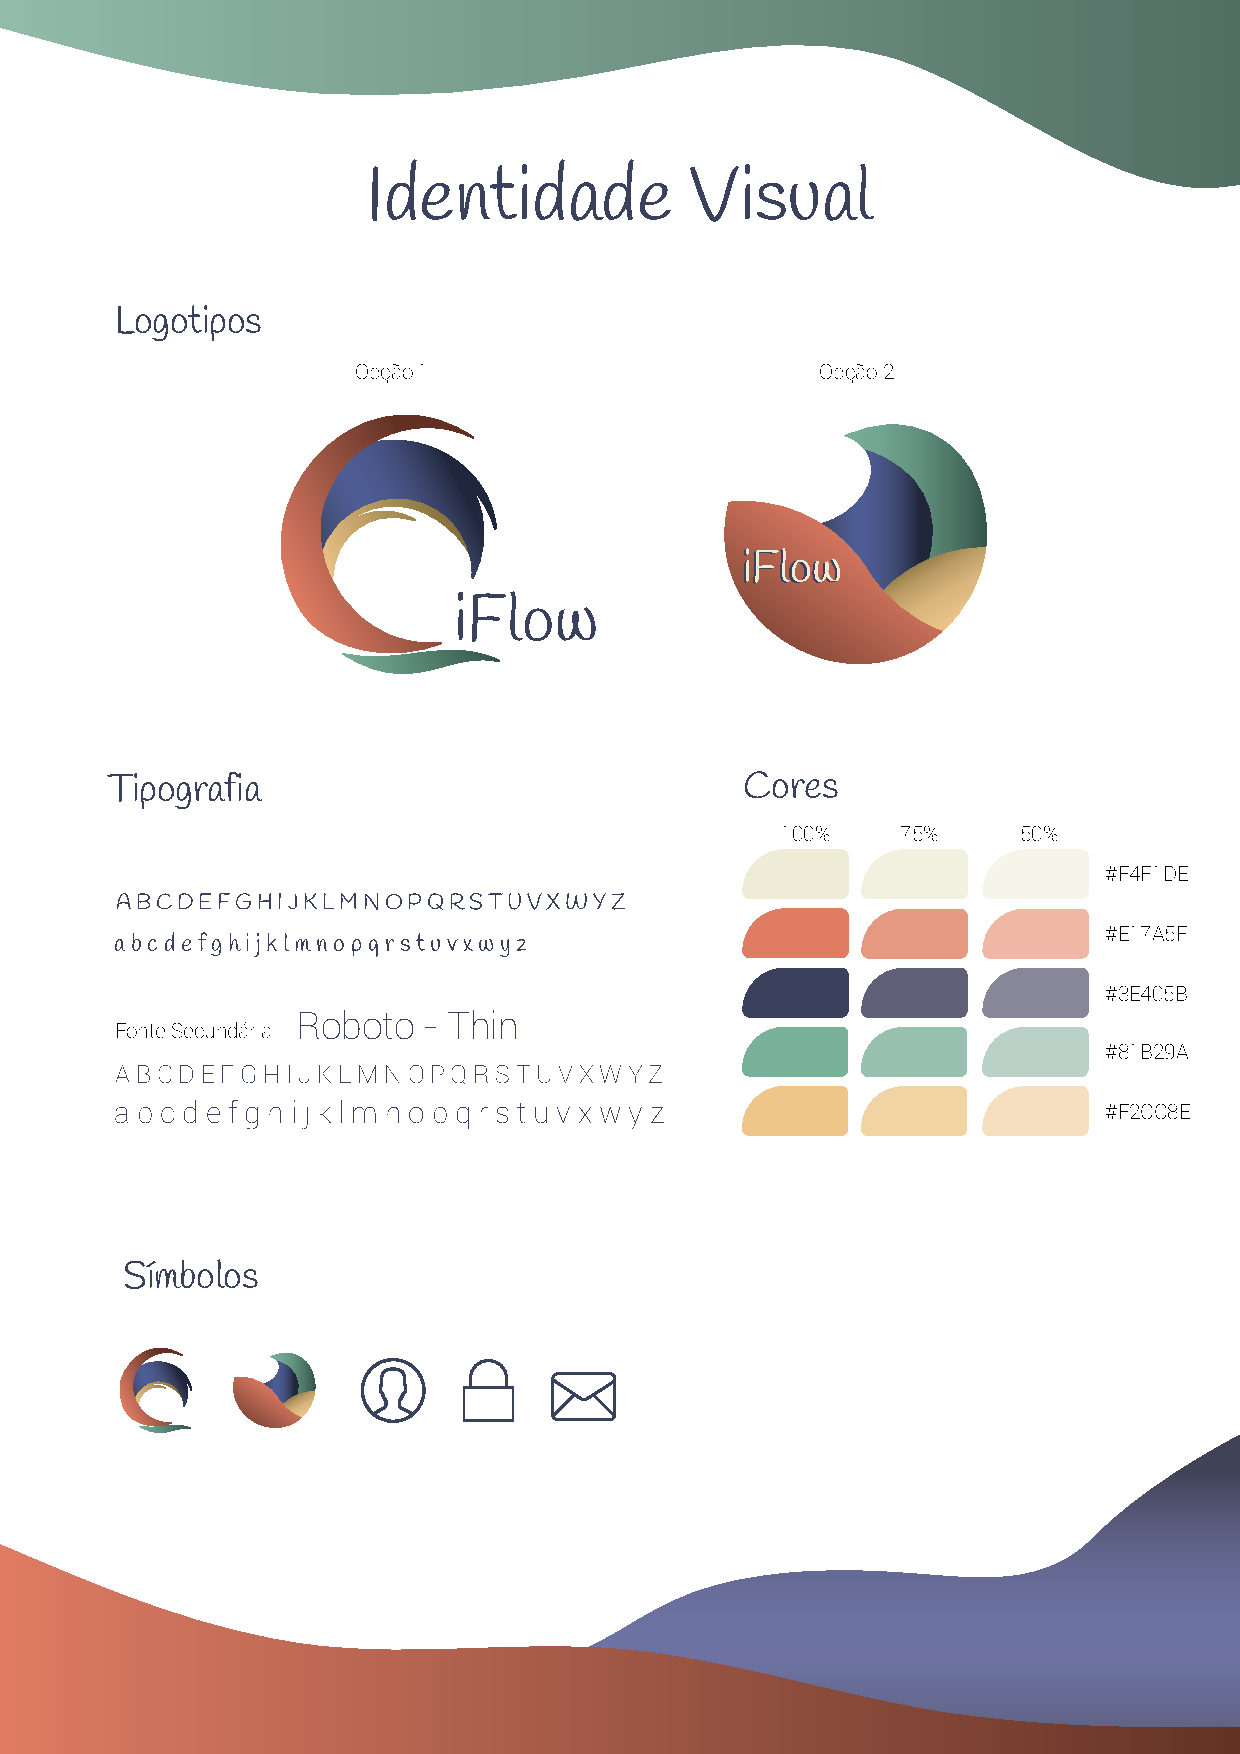
\includepdf[pages={1}]{figuras/Proposta/identidade_visual.pdf}